\subsection{Solving data hazards}
\begin{figure}[!ht]
    \centering
    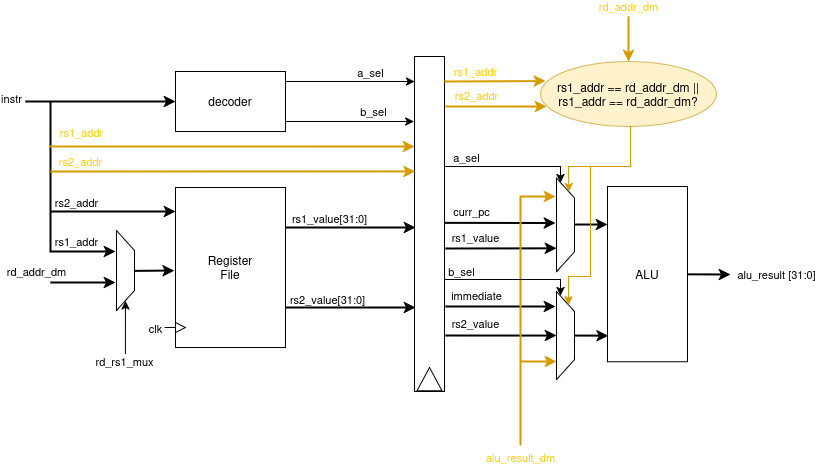
\includegraphics[scale = 0.3]{op_fw_datapath.png}
    \caption{Concept for operand forwarding for solving data hazards}
    \label{fig:op_fw}
\end{figure}

Pipelined architectures change the core system in order to execute instructions partially and with each segment being executed in sequence. This allows for faster clock and a higher throughput, but the fact that each instruction is initiated, in its execution, just a clock cycle later than the previous one introduces a crippling problem regarding the addressing of the same register in consecutive commands, as it happened in the previous simulation (Figure \ref{fig:DPPPL_sim}). This problem can be solved easily by either stalling the pipeline or by passing down the result of the ALU to another stage when needed, also called operand forwarding.
By comparing the destination register of the previous instructions, both in the DM and WB stages, and the operands of the next one, the datapath can be programmed to not increment the PC, thus stalling the pipeline for some clock cycles; Although simple, the solution is wasteful and can lead to slowdowns during very intensive arithmetic operations.
Operand Forwarding could instead have the execution flow just as before and still solve the problem; By adopting the same comparison method, the multiplexers at the ALU's inputs can select the previous result when necessary, and when the same register is addressed multiple times before it can be written, the most recent data can be used.
To successfully implement operand forwarding inside the IE, there is the need to analyze the previous destination register's address that has been passed down to both DM and WB, as said earlier, then confront both of the addresses with the address of each one of the operands and finally overwrite them with the most recent ALU's output. A VHDL description could be given below:

\begin{minted}[fontsize=\footnotesize]{vhdl}
    rs1_fw          <= alu_result_wb when (rd_addr_wb = rs1_addr_in) 
                        else alu_result_dm when (rd_addr_dm = rs1_addr_in)
                        else rs1_value_in;
    rs2_fw          <= alu_result_wb when (rd_addr_wb = rs2_addr_in)
                        else alu_result_dm when (rd_addr_dm = rs2_addr_in) 
                        else rs2_value_in;
    first_operand   <= rs1_fw when a_sel = '1' else curr_pc;
    second_operand  <= rs2_fw when b_sel = '1' else imm_se;
\end{minted}

However this code is incomplete, including the fact that the forwarded value for rs2 has to reach the data memory for the right value to be stored (which can already be dealt with by having \emph{rs2{\_}fw} as output from the IE), the register file will always be written after 3 clock cycles from the execution stage, meaning that there is another stage that must be covered, which is the ID. In this case an additional line can be added in order for the output of the register file to be overwritten if the register that has to be accessed has not been written yet:

\begin{minted}[fontsize=\footnotesize]{vhdl}
    reg : register_file
    port map(
        clk         => clk,
        da          => instr(11 downto 7) when op_class = "000110"  else instr(19 downto 15),
        pda         => instr(24 downto 20),
        dina        => rd_addr_in,
        din         => rd_value,
        we          => rd_write_en,
        rso         => rs1_value_reg,
        prso        => rs1_value_reg);

    rd_addr <= instr(11 downto 7);
    rs1_addr<= instr(19 downto 15);
    rs2_addr<= instr(24 downto 20);
    
    rs1_value_out <= rd_value when (instr(19 downto 15) = rd_addr_wb and rd_write_en = '1') 
                     else rs1_value_reg;
    rs2_value_out <= rd_value when (instr(24 downto 20) = rd_addr_wb and rd_write_en = '1') 
                     else rs1_value_reg;
\end{minted}
With the forwarding logic now ready, the simulation will show that the processor may be able to change the value of the operand with the latest data from other stages, this can be proven by having the store and load operation reading and writing from the same register as happens in the unpipelined datapath simulation.
In Figure \ref{fig:op_fw_sim} the withdrawed register values are shown in yellow, the forwarded values are highligted in orange. The final value used for each operand is shown in red and the results are exactly what expected, with the SW instruction having the ALU's result pointing at the address number 1, since the upper 19 bits of rs2 (containing 65540) are ignored (hence the resulting address should 4) with the first two bits as well, and with LW being able to address the same location in the memory, whose value is shown in the signal at the bottom to be in fact 131076.
\newpage

\begin{figure}[!ht]
    \centering
    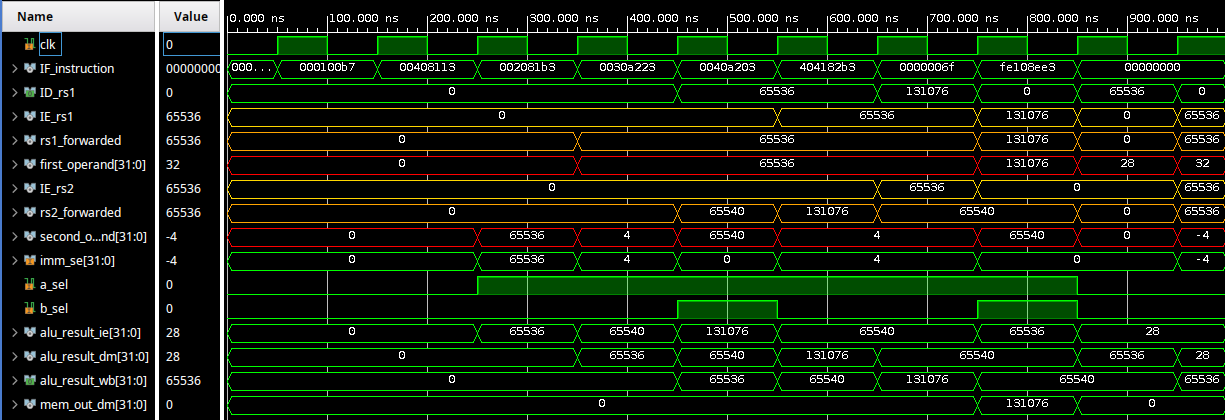
\includegraphics[scale = 0.35]{op_fw_sim.png}
    \caption{Datapath simulation with forwarding logic}
    \label{fig:op_fw_sim}
\end{figure}

\subsection{Managing control hazards}
Managing jumps and branches in a pipelined architecture is not trivial but it is a necessary step to take to achieve a functional processor. Overlooking this feature could lead to incorrect values written in some registers or in the data cache while a jump instruction is being executed. To make an example, the following instruction can be analyzed step by step:
\begin{minted}{gas}
    jal x5, 8           ; PC += 8, x5 = PC + 4    
    add x1, x2, x3      ; x1 = x2 + x3
    sub x4, x1, x3      ; x4 = x1 - x3
\end{minted}
As the first instruction is decoded, the addition is already being fetched and while the PC gets updated just after 4 clock cycles, both the addition and subtraction have been almost fully executed, leading to the content of x4 being updated to the value stored in x2, two cycles after the jump has completed its elaboration and updated the PC, leading to a double execution of the subtraction that also uses a wrong value for x1.
One solution for this would imply that, when the jump is first decoded, the PC has to be kept constant until the jump is fully executed. In addition, all data given by each stage after the jump is first decoded has to be reset (flushed) in order to avoid any unnecessary elaboration. To do this, every register in the pipeline could have a reset input that discards all input values and keeps all outputs to zero; With the current outputs available from the other stages, this is easily doable by having the latter being pulled high when \emph{op{\_}class} = "010000" (unconditional jump) at any stage or when a branch has its condition true, that is, when \emph{branch{\_}cond} = 1.
By looking at the actual code, the first modification that needs to be made is adding a new input to the IF entity that can keep the PC constant until a new value is loaded. The snippet below shows how the PC can interact with the stated modification:

\begin{minted}[fontsize=\footnotesize]{vhdl}
    process (clk)
    begin
        if rising_edge(clk) then
            if pc_stall = '1' then
                pc_reg  <= pc_reg;
            elsif pc_load_en = '1' then
                pc_reg  <= unsigned(pc_in);
            else
                pc_reg <= pc_reg + 4;
            end if;
        end if;
    end process;
\end{minted}

The second crucial modification that has to be introduced is a way to have all the inter-stage registers, in particular the ones before the current elaboration stage of the jump, flushed. Since \emph{op{\_}class} and \emph{branch{\_}cond} are propagated to every stage after decoding, the sole presence of an operation class associated to an unconditional jump, or a true condition for a branch, at any stage should be a sufficient condition for the register to be flushed. For each one of them, Table \ref{table:flush_logic} shows which condition for the flush can be used: 

\begin{table}[!ht]
    \begin{center}
        \begin{tabular}{|c|c|}
            \hline
            IF/ID &  branch{\_}cond{\_}(any stage) = 1 OR op{\_}class{\_}(any stage) = "010000"   \\
            
            ID/IE &  branch{\_}cond{\_}(ie,dm,wb) = 1 OR op{\_}class{\_}(ie,dm,wb) = "010000"   \\
            
            IE/DM & branch{\_}cond{\_}(dm,wb) = 1 OR op{\_}class{\_}(dm,wb)= "010000"\\
            
            DM/WB & branch{\_}cond{\_}(wb) = 1 OR op{\_}class{\_}(wb)= "010000"\\
            
            \hline
        \end{tabular}
    \caption{Flush condition for each inter-stage register}
    \label{table:flush_logic}
    \end{center}
\end{table}
\newpage
An observation that needs to be made before implementing the logic is that aas of now, branch{\_}cond can be high even if there is no branch instruction being executed, for that reason, an additional modification has to be made to the original code of the IE stage:

\begin{minted}[fontsize=\footnotesize]{vhdl}
architecture Structural of instr_exec_pipeline is
    
    -- other signal declarations

    signal branch_cond_buf  : std_logic;

    -- ALU component declaration
    
    component comparator is
        port ( 
            first_operand   : in std_logic_vector(31 downto 0);
            second_operand  : in std_logic_vector(31 downto 0);
            cond_opcode     : in std_logic_vector(2 downto 0);
            
            branch_cond     : out std_logic);
    end component;
begin
    comp : comparator 
    port map(
        first_operand   => rs1_value_in,
        second_operand  => rs2_value_in,
        cond_opcode     => cond_opcode,
        branch_cond     => branch_cond_buf); 
    
    -- forwarding logic and ALU instantiation
    
    branch_cond     <= branch_cond_buf when op_class(5) else '0';
\end{minted}

Source Code \ref{code:IF_ID} shows in the IF/ID register the implementation of a flush input, while Source Code \ref{code:DTPTH_pipelined} shows the statements that drive that input in each register.

